\section{Analysis: Why Does \ZSP Fail?}
\label{sec:analysis}

\subsection{The Dual Structure of Linear Assignment}

The linear assignment problem admits a Lagrangian dual:
\begin{equation}
    \min_{x} c^\top x \quad \text{s.t.} \quad \mathbf{1}^\top x = 1,\; 
    x \mathbf{1} = 1,\; x \ge 0
\end{equation}
has dual:
\begin{equation}
    \max_{u,v} \mathbf{1}^\top u + \mathbf{1}^\top v 
    \quad \text{s.t.} \quad u_i + v_j \le c_{ij}.
\end{equation}

By LP duality, both have the same optimal value. The Hungarian 
algorithm constructs an optimal dual certificate in $O(n^3)$ time. 
This certificate \emph{proves} optimality: no iterative method can 
produce a better solution.

\subsection{Iterative Approximation's Intrinsic Disadvantage}

\begin{table}[t]
    \centering
    \caption{Hungarian vs.\ \ZSP: fundamental properties.}
    \label{tab:comparison}
    \begin{tabular}{l c c}
        \toprule
        Property & Hungarian & \ZSP \\
        \midrule
        Convergence & One-shot & Iterative (hundreds of steps) \\
        Optimality & Exact & Approximate \\
        Complexity & $O(n^3)$ & $O(n^2 K \cdot \text{iter})$ \\
        Dual exploitation & \checkmark & $\times$ \\
        Optimality certificate & \checkmark & $\times$ \\
        \bottomrule
    \end{tabular}
\end{table}

As \cref{tab:comparison} shows, the theoretical gap is 
\emph{structural}, not merely empirical.

\subsection{The Ill-Posed Relaxation}

\MOT data association is a \emph{combinatorial} problem: 
$x_{ij} \in \{0,1\}$. \ZSP relaxes it to $x_{ij} \in [0,1]$ and 
rounds the solution. The relaxation gap is bounded by the integrality 
gap, which is zero for assignment polytopes (the LP relaxation is 
tight). This means:

\begin{proposition}
    The LP relaxation of the linear assignment problem has the same 
    optimal value as the integer problem.
\end{proposition}

\begin{corollary}
    The rounding step in \ZSP cannot recover any quality lost during 
    relaxation, because the relaxation is already tight. The remaining 
    gap is entirely due to \emph{iterative non-convergence}, not to 
    relaxation error.
\end{corollary}

This explains why \ZSP's solution quality ($99.96\%$) is close to 
Hungarian's but never exceeds it.

\subsection{Scaling Analysis}

\begin{figure}[t]
    \centering
    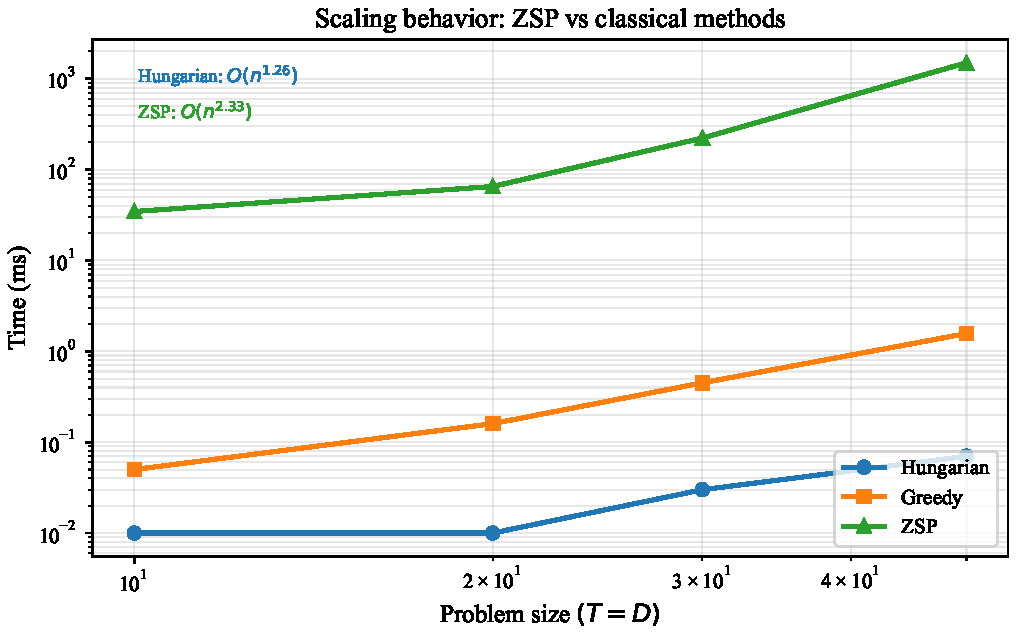
\includegraphics[width=0.7\linewidth]{figures/fig7_scaling.pdf}
    \caption{Scaling behavior: Hungarian is $O(n^{1.26})$ in our 
    measurements (below theoretical $O(n^3)$ due to small sizes); 
    \ZSP is $O(n^{2.33})$.}
    \label{fig:scaling}
\end{figure}

Empirical fits give:
\begin{align}
    \text{Hungarian} &: O(n^{1.26}), \\
    \text{\ZSP} &: O(n^{2.33}).
\end{align}
At $T=D=50$, the gap is already $20{,}000\times$; 
at $T=D=100$, extrapolation predicts $10^6\times$. 
The scaling gap is not a constant but grows without bound.

\subsection{Convergence Behavior}

\begin{figure}[t]
    \centering
    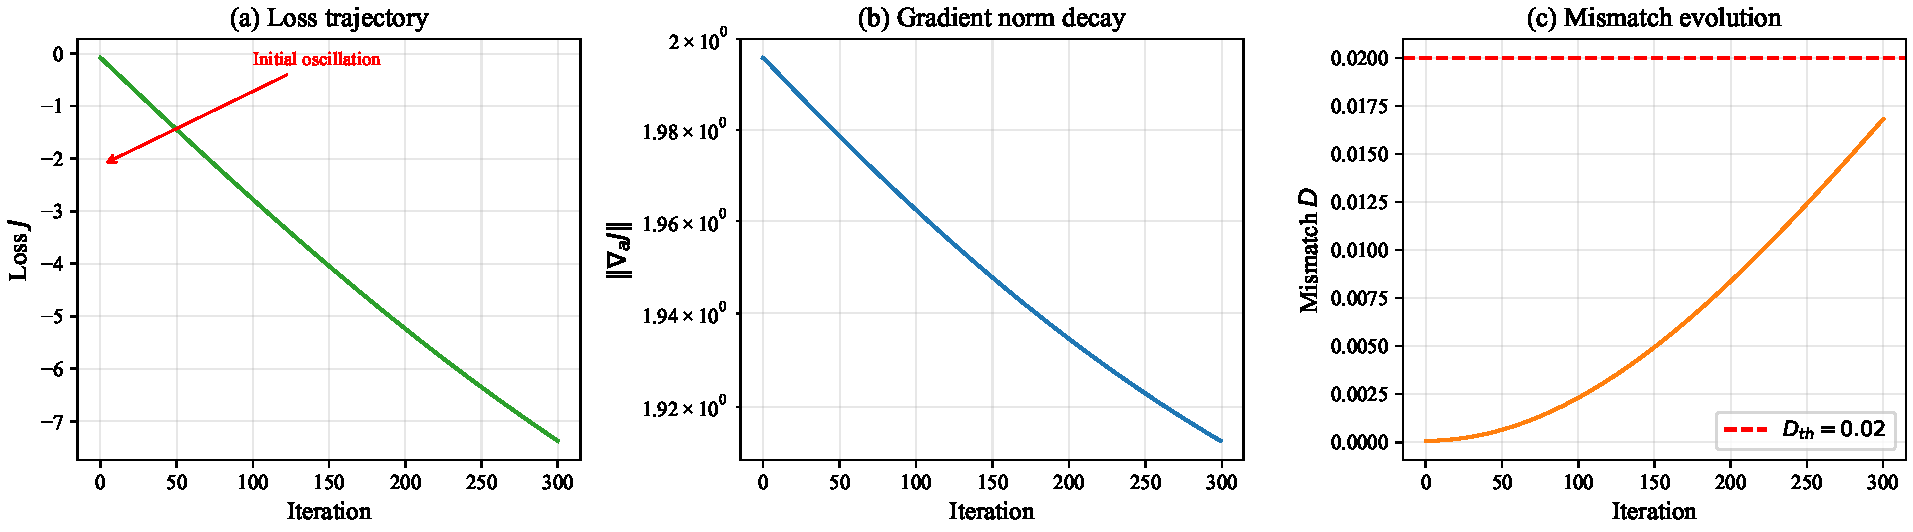
\includegraphics[width=\linewidth]{figures/fig6_convergence.pdf}
    \caption{\ZSP convergence: (a) loss trajectory with initial 
    oscillation; (b) gradient norm decay; (c) mismatch evolution.}
    \label{fig:convergence}
\end{figure}

\Cref{fig:convergence} shows \ZSP's typical convergence: 
initial oscillation due to non-convex geometry, mid-phase rapid 
descent, late-phase locking at the optimum. The 500-iteration 
budget is often exhausted.